\documentclass[green]{GL2020}

\usepackage{array}
\usepackage{xcolor}
\usepackage{hyperref}
\usepackage{multicol}
\usepackage{ltablex}
\usepackage{tabularx}
\renewcommand{\tabularxcolumn}[1]{m{#1}}
\setlength{\columnsep}{1cm}

\usepackage{graphicx}
\graphicspath{ {C:/Users/charf/Documents/GitHub/GL2020/Puzzles/} }


\parindent=0pt
\begin{document}
\name{\gWeekendSchedule{}}

Below is the full event schedule, including both in game and out of game activities as of 29Jul2024. No IC events are mandatory for players to attend. They are probably good places to find other characters, or good times to sneak off and do something secret. The Pre-Game OOC events \textbf{are} mandatory, for the safety and coherence of the event. Post-game OOC events are optional. However, since these activities affect when carpools can leave, players who are carpooling should be prepared to be on site until 5 pm on Sunday, even if they personally wish to opt out of post game workshops.

Dinner on Friday is OOC, as it occurs before the game begins. Time to mingle and socialize as players is important for building rapport that facilitates intense play. This is also a time to do any in person calibration you and your fellow players deem necessary. Dinner on Saturday is also OOC, to give everyone a break. All other meals are optionally in character for soft RP, or OOC, as players choose. We will designate spaces for IC and OOC in the dining hall if it proves valuable.

This schedule is subject to change between now and game start as in and out of game needs mandate. We will have a final copy of the schedule at game, which will supersede this one if any changes are made.

Locations are listed as OOC locations for OOC activities, and IC locations for IC activities. A labeled site map will be provided before game.

%%%%%%%% Meal times: 8 am, 12 pm, 5:30 pm

For workshops on Friday afternoon, please pack a jacket,sunscreen, and bug spray in an easily accessible place in your car/luggage, we may be outside or inside for these, and you may want to grab one or both.

\begin{tabularx}{\textwidth}{|>{\centering\arraybackslash} m{1.6cm} | >{\centering\arraybackslash} m{2cm} | >{\centering\arraybackslash} m{1.8cm} | >{\centering\arraybackslash}X |}
 \hline
\multicolumn{4}{|c|}{\textbf{Friday (Mandatory Pre-Game Activities) 12:00 pm}} \\
\hline 
 \emph{Time} & \emph{Location} & \emph{Event} & \emph{Description}\\
\hline
 12:00 pm - 1:00 pm   & The Cedars & Registration &  Players will check in with the logistics team. Hard copies of game material will be provided. Either eat on the way to the venue, or bring food for a picnic lunch. \\
    \hline
  1:00 pm - 1:15 pm  & The Cedars & Workshop Orientation & Introduction to Workshops. The workshops are designed to help players get into character, create shared cultural touchpoints, and foster trust among players. \\
    \hline
  1:15 pm - 1:45 pm & The Cedars & Logistics Briefing & Logistics team will review camp and game policies with all players. \\
    \hline
  1:50 pm - 3:20 pm & The Cedars & Safety, Calibration, and Combat & This workshop will cover safety mechanics, how calibration and negotiation are used in this game, and practice the combat mechanic.\\
 \hline
  3:25 pm - 4:25 pm &  The Cedars & Workshop by Cohort & Players will have a chance to interact with others in their cohort before game. \\ 
 \hline
  4:30 pm - 5:00 pm & The Cedars & Workshop by Country & Players will have a chance to interact with others in their nation before game. \\
 \hline
 5:00 pm - 6:00 pm & Cedars, Retreat Center  & Load-in \textbf{AND} Costume Time & Time for players to unpack from cars into sleeping spaces. Please also take this time to get into costume, settle in, ask GMs last minute questions, and otherwise get ready for game. \\
 \hline
  6:00 pm - 7:00pm & The Cedars Dining Hall & Dinner. & Please eat food! This is also time to hang out and do any calibration you need to with other players you haven't had a chance to interact with before this point. If you need extra costuming time, feel free to leave dinner early. Please return to the Cedars Lounge by 7 pm. \\
	\hline
\multicolumn{4}{|c|}{\textbf{GAME ON 7:00 pm}} \\
\hline 
7:00 pm & The Great Hall & Game Starts & \cPrincipal{\full} should have a few words to say to start the ``Time of Deciding.’’ \\
 \hline
  8:30 pm - 8:45 pm & The Cohort Lounges/ Bunkers & First Storm Surge & Characters should probably take shelter in the bunkers. Traditionally characters shelter by country during this surge. \\
\hline
  10 pm & Everywhere & Quiet Hours Start & Quiet Hours start now. GM HQ closes for the night.\\
\hline
  12 am & Everywhere  & Game Off & Please get some sleep. \\
    \hline
 \end{tabularx}
  

\begin{tabularx}{\textwidth}{|>{\centering\arraybackslash} m{1.6cm} | >{\centering\arraybackslash} m{2cm} | >{\centering\arraybackslash} m{1.8cm} | >{\centering\arraybackslash}X |}
\hline
\multicolumn{4}{|c|}{\textbf{Saturday}} \\
 \hline
\emph{Time} & \emph{Location} & \emph{Event} & \emph{Description}\\
\hline
  8:30 am - 9:30 am & The Cedars Dining Hall & Breakfast & Please eat food! This meal is optionally available for soft RP.  \\
\hline
  9:20 am - 9:30 am & The Cedars Dining Hall & Game Announcements & GMs may have game related announcements (IC or OOC) at this time, so please plan to attend.  \\
\hline
\multicolumn{4}{|c|}{\textbf{GAME ON 9:30 am}} \\
\multicolumn{4}{|c|}{(Players are welcome to take time after official game start to put on costumes and makeup.)} \\
\hline 
  10:30 am - 11:00 am  &  The Great Hall & Scientific Presentation & \cHeadScientist{\full} and \cAssistantScientist{\full} are scheduled to present the details of the ongoing research into ending the Storms for good.\\
 \hline
  12:30 pm - 1:30 pm & The Cedars Dining Hall & Lunch & Please eat food! This meal is optionally available for soft RP. \\
 \hline
  2:30 pm - 2:45 pm & The Cohort Lounges/ Bunkers & Second Storm Surge & Characters should probably take shelter in the bunkers. Traditionally characters shelter by job cohort during this surge. \\
\hline
  4:30 pm - 5:00 pm &  The Great Hall & Ceremony of Excellence & \cMusic{\full} is in charge of organizing the Ceremony of Excellence to showcase the talent at the school. Characters are encouraged, but not mandated, to attend.  \\
\hline
 6:00 pm - 7:00 pm & The Cedars Dining Hall & Dinner & Please eat food! This meal is \textbf{mandatorily OOC}. There will be an optional personal reflection and expectation management activity available.\\
\hline
  10 pm & Everywhere & Quiet Hours Start & Quiet Hours start now. GM HQ closes for the night.\\
\hline
  12 am & Everywhere & Game Off & Please get some sleep. \\
\hline
\end{tabularx}

\begin{tabularx}{\textwidth}{|>{\centering\arraybackslash} m{1.6cm} | >{\centering\arraybackslash} m{2cm} | >{\centering\arraybackslash} m{1.8cm} | >{\centering\arraybackslash}X |}
\hline
\multicolumn{4}{|c|}{\textbf{Sunday}} \\
\hline
\emph{Time} & \emph{Location} & \emph{Event} & \emph{Description}\\
\hline
8:30 am - 9:30 am & The Cedars Dining Hall & Breakfast & Please eat food! This meal is optionally available for soft RP.  \\
\hline
9:20 am - 9:30 am & The Cedars Dining Hall & Game Announcements & GMs may have game related announcements (IC or OOC) at this time, so please plan to attend.  \\
\hline
\multicolumn{4}{|c|}{\textbf{GAME ON 9:30 am}} \\
\multicolumn{4}{|c|}{(Players are welcome to take time after official game start to put on costumes and makeup.)} \\
\hline
10:30 am - 10:45 am  & The Cohort Lounges/ Bunkers & Third Storm Surge & Characters should probably take shelter in the bunkers. There is no traditional grouping for this surge. \\
\hline
  12:00 pm (noon) & The Great Hall & Votes to Direct the Storm Due, Pedestals Lock Down & Students must submit their votes for where to send the storm by this time, else they will be forfeit. Relics must be placed on pedestals before this time. No changes will be allowed afterwards. .\\
\hline
  12:30 pm - 1:30 pm & The Cedars Dining Hall & Lunch & Please eat food! This meal is optionally available for soft RP.   \\
 \hline
  1:45 pm - 2:15 pm & The Great Hall & Ritual To Control the Storm & The actual ritual to control where the storm is sent will happen at this time.\\
\hline
\multicolumn{4}{|c|}{\textbf{GAME ENDS 2:30 pm}} \\
\hline
\end{tabularx}

\begin{tabularx}{\textwidth}{|>{\centering\arraybackslash} m{1.6cm} | >{\centering\arraybackslash} m{2cm} | >{\centering\arraybackslash} m{1.8cm} | >{\centering\arraybackslash}X |}
\hline
\multicolumn{4}{|c|}{\textbf{Sunday (Optional Post-Game Activities) 2:30 pm}} \\
\hline
2:30 pm - 2:50 pm & The Cedars Lounge & Derole-ing Exercise & Players may choose to join us for a guided activity to begin separating the player from the character and begin processing the weekend. Alternately, players may choose to help with tear down, or reflect alone.\\
 \hline
  2:50 - 4:00 pm & The Cedars Lounge & Game Wrap Up and Goodbyes & Players may choose to join us for a structured wrap-up for game. The GMs will sketch a few key epilogue pieces, and players will be able to share some of their character's story.\\
 \hline
  4:00 to 5:00 pm & Everywhere & Tear Down and Load Out & We will finish cleaning up and loading out from game! Once everyone in your carpool is packed out, cars may leave at any time, although the GMs would appreciate help cleaning up game too.  \\
 \hline
  5:00 pm & Everywhere & Event End & Drive safely on your way home! Everyone must be off-site by 5 pm.  \\
	\hline
\end{tabularx}
\clearpage

\center
{\LARGE Site Map}\\
\vspace{0.5cm}
\begingroup
\vfill
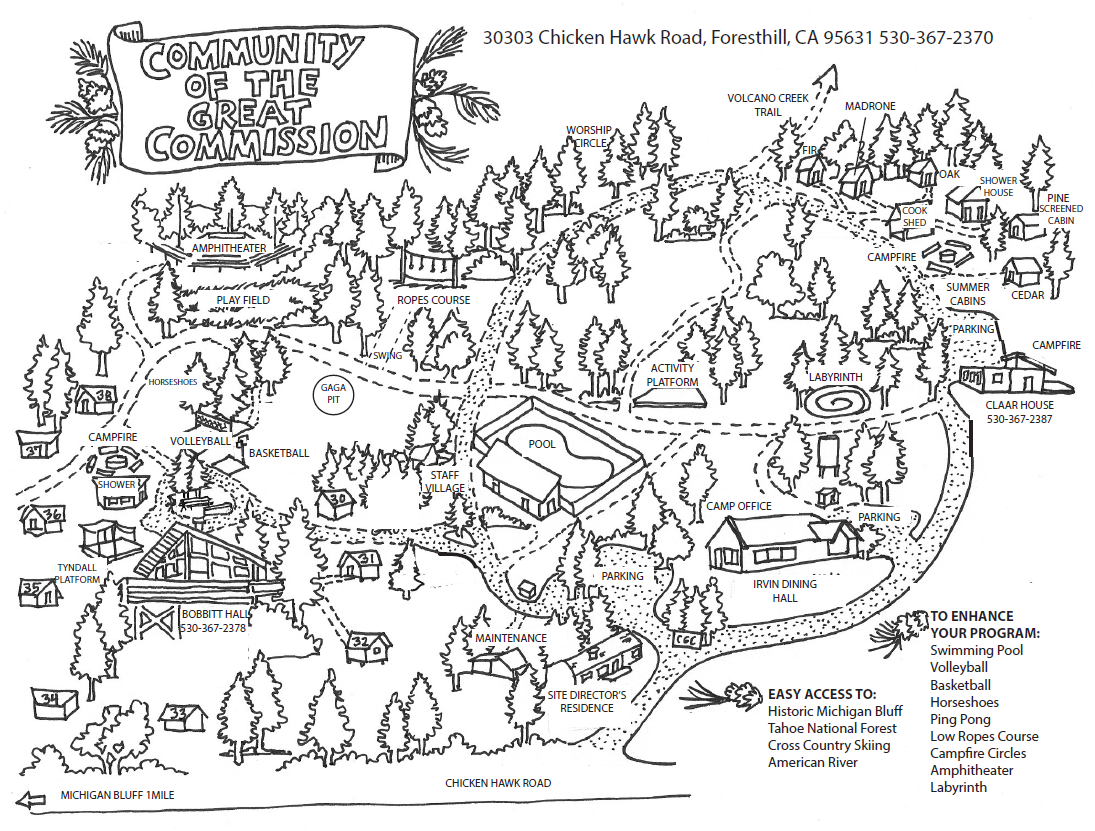
\includegraphics[origin=c,scale=1.1]{SiteMap}
\vfill
\endgroup
\endcenter




\end{document}

